\documentclass{beamer}
\usetheme{Madrid}
\usecolortheme{default}
\usepackage[utf8]{vietnam}
\usepackage[backend=biber,natbib=true,style=alphabetic,maxbibnames=50]{biblatex}
\addbibresource{/home/nqbh/reference/bib.bib}
\usepackage{amsmath,amssymb,amsthm,enumitem,float,graphicx,mathtools,tikz}
\title{Mathematical Methods for Machine Learning\\Phương Pháp Toán Cho Học Máy}
\author{\sc Nguyễn Quản Bá Hồng}
\institute{UMT, HCMC -- University of Management \& Technology, Ho Chi Minh City}
\logo{
\includegraphics[height=5mm]{UMT_logo}}
\date{\today}

\begin{document}
\frame{\titlepage}
\begin{frame}
	\frametitle{Table of Contents}
	\tableofcontents
\end{frame}

\section{Preliminaries}

\begin{frame}
	\frametitle{Resources}
	[Tie20] {\sc Vũ Hữu Tiệp}. {\it Machine Learning Cơ Bản}.
	\vspace{2mm}
	
	[DFO23] {\sc Marc Peter Deisenroth, A. Aldo Faisal, Cheng Soon Ong}. {\it Mathematics for Machine Learning}. 2023.
\end{frame}

\begin{frame}
	\frametitle{Audiences \& Goals}
	{\bf Target Audience.} Mainly: Engineering- \& CS undergraduate students.
	
	\underline{Note}: Mathematics undergraduate students, especially academic-oriented (researchers), need much more rigorously theoretical mathematical foundations for ML.	
	\begin{block}{Goal{\tt/}Objective}
		Learn enough mathematics to be able to balance our comprehension in both mathematical- \& technical (engineering) aspects of Machine Learning: Adjust ``suitable'' coefficients $\alpha,\beta,\gamma\in(0,1)$ s.t. $\alpha + \beta + \gamma = 1$ \&
		\begin{equation}
			 \boxed{\mbox{Maximize } {\rm Goal}({\rm What,How,Why})\coloneqq\alpha{\rm What} + \beta{\rm How} + \gamma{\rm Why}.}
		\end{equation}
		where the functional ${\rm Goal}({\rm What,How,Why})$ depends on your target job(s) \& purpose(s).
	\end{block}
\end{frame}

\begin{frame}
	\frametitle{Audiences \& Goals}
	Distinguish 2 different perspectives{\tt/}orientations for a CS student: Engineering-oriented \& Mathematics-oriented.
	\begin{block}{Engineering perspective}
		Engineers need to learn various What (definitions, tools) \& mainly focus on How (technicalities, tools), ``practical Why'' \& a little bit on ``theoretical Why''.
	\end{block}
	E.g.: {\it Why does this algorithm{\tt/}model work? Why does(n't) my code work?}
	
	\begin{block}{Mathematics perspective}
		Mathematicians have to learn \& build various What (definitions, concepts), mainly focus on ``theoretical Why'' (logic, rigorous proof), then on How (mathematical tools)
	\end{block}
	E.g.: {\it Why is this model ``optimal'' in mathematical sense?}
\end{frame}

\begin{frame}
	\frametitle{Prerequisites}
	\begin{figure}[H]
		\centering
		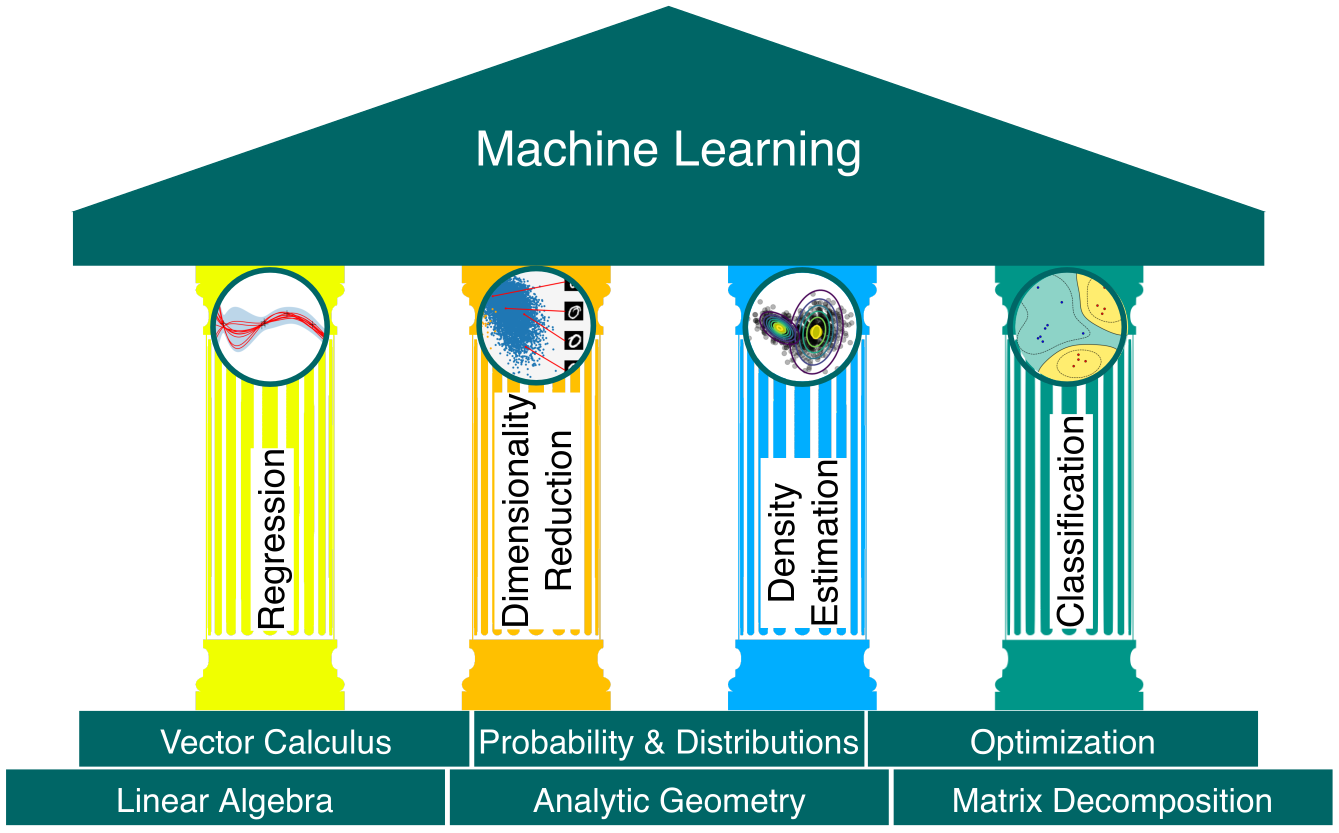
\includegraphics[width=10cm]{4_ML_pillars}
		\caption{Foundations \& 4 pillars of ML. Source: \cite[Fig. 1.1, p. 14]{Deisenroth_Faisal_Ong2023}.}
	\end{figure}
	
\end{frame}

\begin{frame}
	\frametitle{Prerequisites}
	\begin{itemize}
		\item Linear Algebra
		\item Probability
		\item Statistics
	\end{itemize}
\end{frame}

\section{Basic Mathematics for Machine Learning}

\begin{frame}
	\frametitle{Artificial Neural Networks (ANNs)}
\end{frame}

\section{Advanced Mathematics for Machine Learning}
	
\end{document}